%CHE EZE, COMO VISTE ESTE COMENTARIO? SI TE DIMOS UN PDF
%ANDY LA CONCHA DE TU MADRE, Joaco tonto
\documentclass[titlepage,a4paper]{article}
\usepackage{a4wide}
\usepackage[colorlinks=true,linkcolor=black,urlcolor=blue,bookmarksopen=true]{hyperref}
\usepackage{bookmark}
\usepackage{fancyhdr}
\usepackage[spanish]{babel}
\usepackage[utf8]{inputenc}
\usepackage[T1]{fontenc}
\usepackage{textcomp, gensymb}
\usepackage{graphicx}
\usepackage{float}
\usepackage{multicol}

\pagestyle{fancy} % Encabezado y pie de página
\fancyhf{}
\fancyhead[L]{TP2 - Grupo 1}
\fancyhead[R]{Análisis Numérico - FIUBA}
\renewcommand{\headrulewidth}{0.4pt}
\fancyfoot[C]{\thepage}
\renewcommand{\footrulewidth}{0.4pt}
\usepackage[utf8]{inputenc}

\begin{document}
\begin{titlepage} % Carátula
	\hfill
\includegraphics[width=6cm]{logofiuba.jpg}
    \centering
    \vfill
    \Huge \textbf{Trabajo Práctico 2}
    \vskip2cm
    \Large [ 75.12 - 95.04 ] Análisis Numérico\\
    Curso 5 \\ 
    Primer cuatrimestre de 2020\\
    \vfill
    \begin{tabular}{ | l | l | } 
      \hline
        De Angelis Riva, Lukas & 103784 \\ \hline
        Gomez, Joaquín & 103735 \\ \hline
        Grassano, Bruno & 103855 \\ \hline
        Guillemi, Andrés & 104006\\ \hline 
        Rodríguez, Ezequiel & 103976 \\ \hline
        Romero, Adrián & 103371 \\ \hline
  	\end{tabular}
    \vfill
    \vfill
    \vfill
\end{titlepage}

\tableofcontents % Índice general
%BOQUITA EL MAS GRANDE PAPA
\newpage

\section{Introducción}\label{sec:intro}
    En el presente trabajo práctico tenemos como objetivo crear un programa para la resolución de una ecuación diferencial de segundo orden con coeficientes constantes, que describe la posición y la velocidad de un péndulo, a través de los siguientes métodos numéricos aprendidos a lo largo de la materia:
    \begin{itemize}
        \item Runge-Kutta de orden 1 (Euler)
        \item Runge-Kutta de orden 4
    \end{itemize}
    
    Con este fin, creamos un programa en Python que nos permite calcular las constantes necesarias para realizar las iteraciones de estos métodos. Luego procedimos a calcular y graficar los resultados obtenidos para posición, velocidad y energía en un intervalo de 20 segundos.

\section{Objetivos}\label{sec:objetivos}
    El objetivo del trabajo es resolver una ecuación diferencial por medio de los métodos indicados anteriormente, para distintos pasos $h$ y comparar los órdenes de error. 
    
    Además pretendemos estudiar el comportamiento de la energía $E$ para distintos tipos de amortiguamientos $b$.


\section{Análisis previo}
    La siguiente es la ecuación diferencial que describe el ángulo de un péndulo simple $\theta$ en función del tiempo $t$ para las condiciones iniciales $\theta_0$ y $\theta'_0$:
    
    \begin{center}
        EDO: \hspace{2mm} $\frac{d^2\theta}{dt^2}+\frac{b}{m}\frac{d\theta}{dt} +\frac{g}{l}\theta = 0$ \hspace{5mm} CI: \hspace{2mm} $\theta(0) = \theta_0$ \hspace{3mm} $\frac{d\theta}{dt}(0) = \theta'_0$
    \end{center}
    
    Dado que es una ecuación diferencial de segundo orden, para poder aplicar los métodos de RK1 y RK4, es necesario realizar un cambio de variables $u = \theta'$, resulta entonces:
    
    \begin{center}
        EDOS: \hspace{2mm} $\theta' = u$ \hspace{15mm} CI: \hspace{2mm} $\theta(0) = \theta_0$ \\
        \hspace{15mm}$u' = -\frac{b}{m}u-\frac{g}{L}\theta$ \hspace{10mm} $u(0) = u_0$
    \end{center}
    
    Donde llamando $f(t, \theta, u) = -\frac{b}{m}u-\frac{g}{L}\theta$ podemos plantear los metodos de la siguiente manera:
        
    Runge-Kutta 1:
    
    \begin{center}
        $u_{n+1} = u_{n} + h \cdot f(t_n, \theta_n, u_n)$\\
        $\theta_{n+1+} = \theta_{n} + h \cdot u_n$
    \end{center}
    
    Runge-Kutta 4:
    
    \begin{center}
        $u_{n+1} = u_{n} + \frac{h}{6} ( m_1 + 2m_2 + 2m_3 + m_4)$\\
        $\theta_{n+1+} = \theta_{n} + \frac{h}{6}  ( k_1 + 2k_2 + 2k_3 + k_4)$
    \end{center}
    
    Donde las constantes $k$ y $m$ cumplen:
    
    \begin{multicols}{2}
    \centering
    $k_1 = u_n$\\
    $k_2 = u_n + \frac{1}{2}hm_1$\\
    $k_3 = u_n + \frac{1}{2}hm_2$\\
    $k_4 = u_n + hm_3$\\
    \columnbreak
    $m_1 = f(t_n, \theta_n, u_n)$\\
    $m_2 = f(t_n +\frac{1}{2}h, \theta_n+\frac{1}{2}hm_1, u_n+\frac{1}{2}hk_1)$ \\
    $m_3 = f(t_n +\frac{1}{2}h, \theta_n+\frac{1}{2}hm_2, u_n+\frac{1}{2}hk_2)$ \\
    $m_4 = f(t_n +h, \theta_n+hm_3, u_n+hk_3)$ \\
    \end{multicols}

\newpage

\section{Resultados}

    En las siguientes secciones, mostraremos las soluciones aproximadas de la ecuación diferencial anterior, halladas por los método de Runge-Kutta 1 y 4, y para distintos sets de parámetros: $b$, $m$, $L$, $\theta_0$, $\theta'_0$ y $h$.
    
    Se muestran los primeros y los últimos cinco valores obtenidos para $\theta$ y $\theta'$.
    
    \subsection{Caso 1: Sistema no amortiguado}
    
    \begin{center}
        m = 1kg \hspace{3mm}
        L = 1m \hspace{3mm}
        b = 0 $Nsm^-1$ \hspace{3mm}
        h = 0.02s \hspace{3mm}
        $\theta_0$ = $30\degree$ \hspace{3mm}
        $\theta'_0 = 0\frac{\degree}{s}$ \hspace{3mm}
    \end{center}
    
    \begin{center}
        \begin{tabular}{| c | c | c | c | c | c|}
            \hline
           Tiempo[s] &\multicolumn{2}{|c|}{$\theta_n[rad]$} &\multicolumn{2}{|c|}{$\theta'[rad/s]$} \tabularnewline
            \hline
            &RK1&RK4&RK1&RK4\\
            \hline
            0.00&5.236e-01&5.236e-01&0.000e+00&0.000e+00\\
            0.02&5.236e-01&5.226e-01&-1.026e-01&-1.026e-01\\
            0.04&5.215e-01&5.195e-01&-2.053e-01&-2.047e-01\\
            0.06&5.174e-01&5.144e-01&-3.075e-01&-3.061e-01\\
            0.08&5.113e-01&5.073e-01&-4.089e-01&-4.062e-01\\
            ...&...&...&...&...\\
            19.92&3.125e+00&4.663e-01&6.048e+00&7.4058e-01\\
            19.94&3.246e+00&4.802e-01&5.435e+00&6.530e-01\\
            19.96&3.555e+00&4.924e-01&4.779e+00&5.577e-01\\
            19.98&3.451e+00&5.025e-01&4.142e+00&4.602e-01\\
            20.00&3.534e+00&5.100e-01&3.465e+00&3.600e-01\\
            \hline
        \end{tabular}
        
        \smallskip
        Tabla mostrando los datos correspondientes al sistema no amortiguado
    \end{center}

\subsection{Caso 2: Sistema amortiguado}

    \begin{center}
        m = 1kg \hspace{3mm}
        L = 1m \hspace{3mm}
        b = 0.5 $Nsm^-1$ \hspace{3mm}
        h = 0.02s \hspace{3mm}
        $\theta_0$ = $30\degree$ \hspace{3mm}
        $\theta'_0 = 100\frac{\degree}{s}$ \hspace{3mm}
    \end{center}
    
    \begin{center}
        \begin{tabular}{| c | c | c | c | c | c|}
            \hline
           Tiempo[s] &\multicolumn{2}{|c|}{$\theta_n[rad]$} &\multicolumn{2}{|c|}{$\theta'[rad/s]$} \tabularnewline
            \hline
            & RK1 & RK4 & RK1 & RK4 \\
            \hline
            0.00 & 5.236e-01 & 5.236e-01 & 1.745e+00 & 1.745e+00\\
            0.02 & 5.585e-01 & 5.573e-01 & 1.625e+00 & 1.623e+00\\
            0.04 & 5.910e-01 & 5.885e-01 & 1.500e+00 & 1.495e+00\\
            0.06 & 6.210e-01 & 6.170e-01 & 1.369e+00 & 1.362e+00\\
            0.08 & 6.484e-01 & 6.429e-01 & 1.233e+00 & 1.226e+00\\
            ...&...&...&...&...\\
            19.92 & 1.041e-02 & 2.460e-04 & 1.123e-01 & 1.702e-02\\
            19.94 & 1.265e-02 & 5.841e-04 & 1.091e-01 & 1.677e-02\\
            19.96 & 1.483e-02 & 9.165e-04 & 1.055e-01 & 1.646e-02\\
            19.98 & 1.694e-02 & 1.242e-03 & 1.016e-01 & 1.609e-02\\
            20.00 & 1.897e-02 & 1.560e-03 & 9.722e-02 & 1.565e-02\\
            \hline
        \end{tabular}
        
        \smallskip
        Tabla mostrando los datos correspondientes al sistema amortiguado
    \end{center}
    
    \newpage
    
    \subsubsection{Gráficos}
    A continuación procederemos a mostrar los gráficos representativos a los valores obtenidos en las tablas de la sección anterior. De estos haremos una reflexión en la sección \ref{sec:conclusiones}.
    
    Decidimos no quitar los gráficos de Euler para el caso en que no hay amortiguamiento para denotar cómo funcionan ambos métodos y no alterar las conclusiones del informe.
    
    \begin{figure}[H]
        \centering
        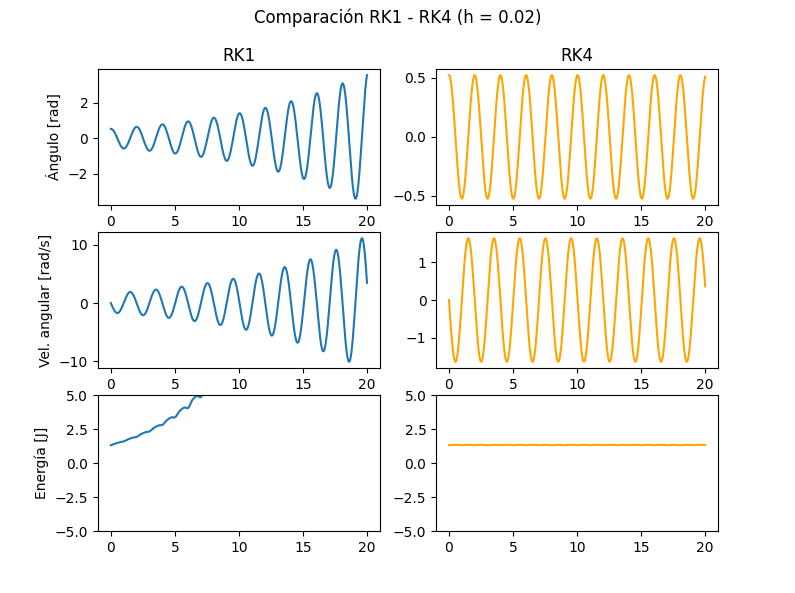
\includegraphics[scale = 0.4]{noAmortiguado1.png}
        \caption{Gráficos mostrando los métodos de Runge-Kutta 4 y Euler para el primer caso en que no hay amortiguamiento}
    \end{figure}
    
    \begin{figure}[H]
        \centering
        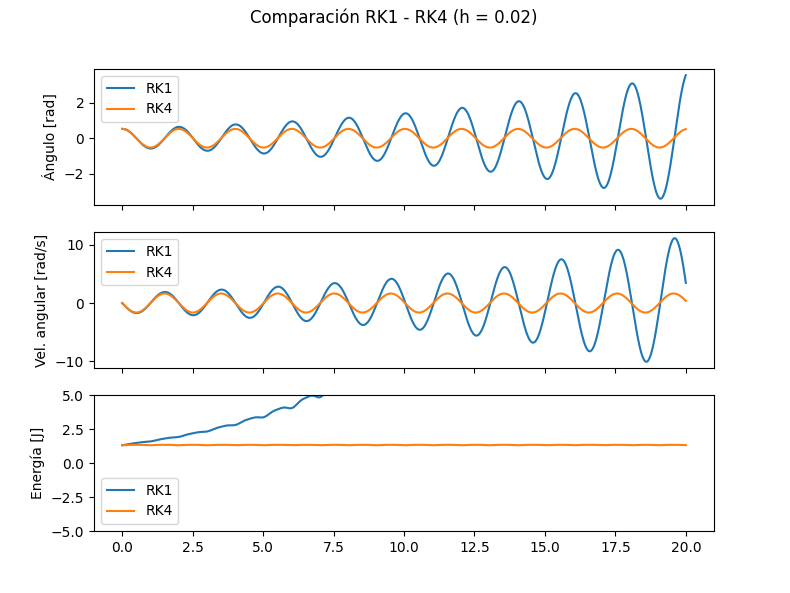
\includegraphics[scale = 0.4]{noAmortiguado2.png}
        \caption{Gráfico mostrando ambos métodos superpuestos}
        \label{fig:noAmortiguadoGrafJuntos}
    \end{figure}
    
    \begin{figure}[H]
        \centering
        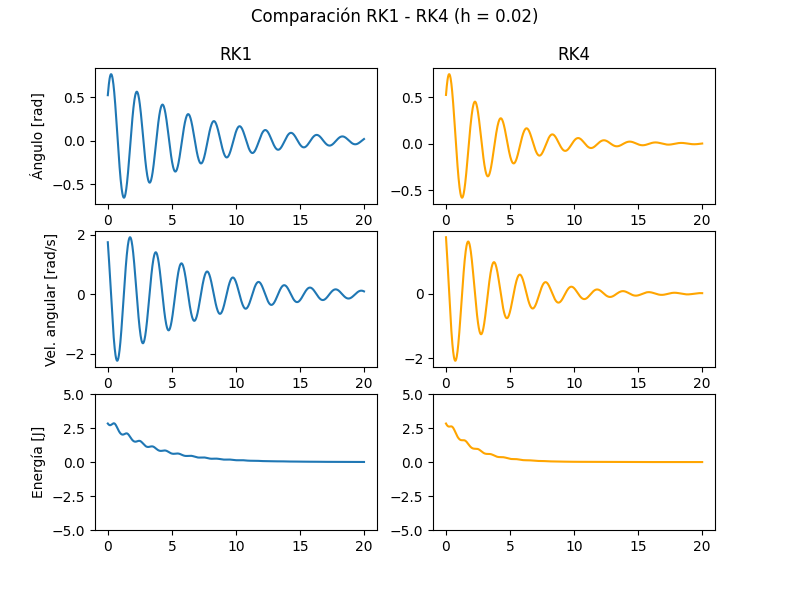
\includegraphics[scale = 0.4]{amortiguado1.png}
        \caption{Gráficos mostrando los métodos de Runge-Kutta 4 y Euler para el segundo caso en que hay amortiguamiento}
    \end{figure}
    
    \begin{figure}[H]
        \centering
        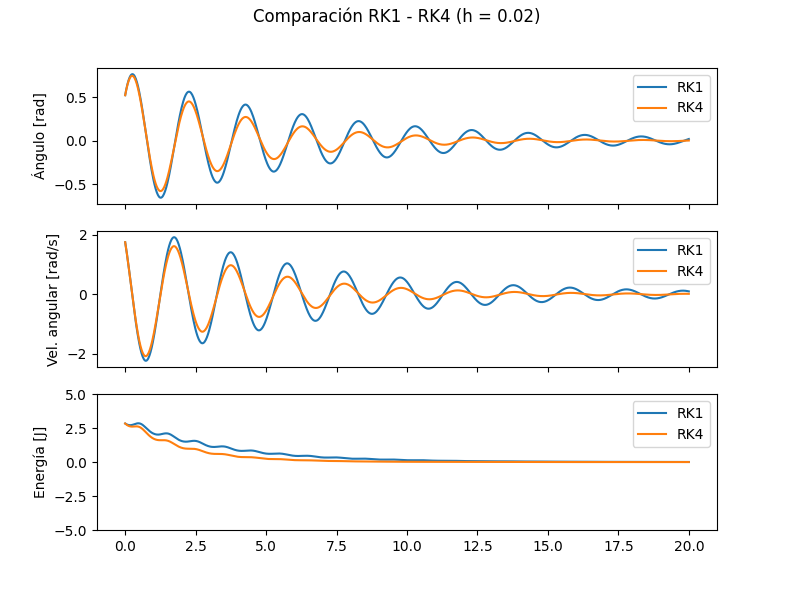
\includegraphics[scale = 0.4]{amortiguado2.png}
        \caption{Gráfico mostrando ambos métodos superpuestos}
    \end{figure}

\newpage

\section{Conclusiones}\label{sec:conclusiones}
    Detallamos a continuación las conclusiones que fueron surgiendo a lo largo del trabajo práctico. Tomamos como solución real la alcanzada mediante RK4 con un paso muy pequeño (h=0.00002)
    
    \begin{figure}[!htb]
        \centering
        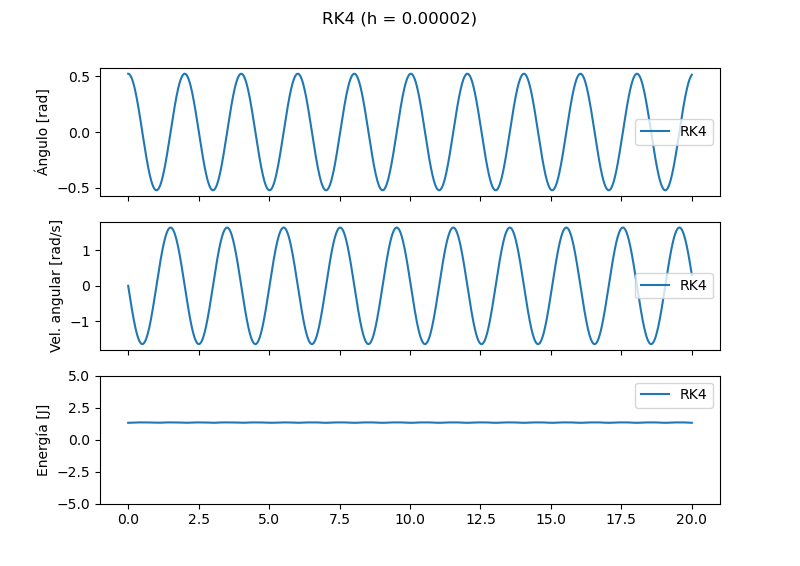
\includegraphics[scale = 0.7]{GraficosRK4/rk4_00002 no amortiguado.png}
        \caption{RK4 no amortiguado h = 0.00002}
    \end{figure}
    
    \begin{figure}[!htb]
        \centering
        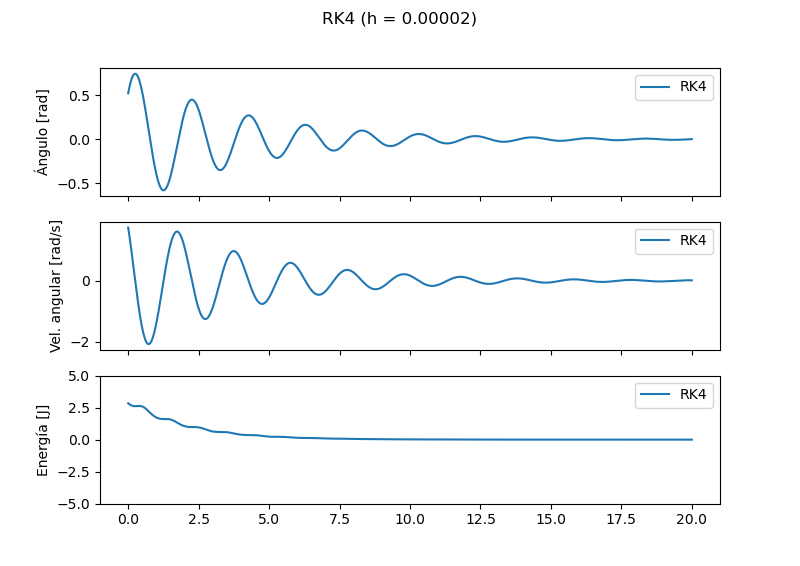
\includegraphics[scale = 0.6]{GraficosRK4/rk4_00002_amortiguado.png}
        \caption{RK4 amortiguado h=0.00002}
    \end{figure}
    
    \begin{itemize}
    
    \newpage

        \item Caso 1:
        \begin{itemize}
            \item Ángulo:
            
        Para el método de Euler la estimación no tiene sentido físico, el ángulo supera al inicial siendo que la velocidad inicial es nula. Esto es imposible y atribuimos el error al tipo de ecuación y al método que utilizamos para resolverla.
            
            Para el método de Runge-Kutta 4 la estimación fue representativa físicamente, al no haber coeficiente de amortiguamiento el péndulo se debería comportarse de manera ideal y así fue, pues la función del el ángulo en función del tiempo tiene forma cosenoidal.

            
            \item Velocidad angular:
            
            Para el método de Euler la estimación carece nuevamente de sentido físico, pues sin acción de una fuerza externa la velocidad angular del péndulo está aumentando el máximo valor, y esto es imposible. Nuevamente consideramos que este error se debe a la ecuación y al método que estamos utilizando para resolverla.
            
            Para el método de Runge-Kutta 4 la estimación nuevamente es representativa físicamente, por lo mismo que comentamos antes, dado que no hay fuerza externa al modelo que actúe sobre él, la velocidad debería mantenerse acotada como se pudo observar correctamente. 


            \item Energía:
            
            Idealmente en el caso no amortiguado no existe disipación de energía, ya que se trata de un sistema cerrado en el cual no existen fuerzas además de la fuerza peso (fuerza conservativa) y la tensión de la cuerda (la misma realiza trabajo nulo ya que es ortogonal al desplazamiento), por lo que el trabajo realizado es igual a cero.  Esto se debería ver reflejado obteniendo un gráfico constante para la energía.  Sin embargo, la energía no se comportó como esperábamos en el método de Euler, pues la energía comenzó a crecer con el tiempo lo cual es físicamente imposible.
            
            Esto puede deberse a diversos motivos.
            Por ejemplo: puede deberse a que la ecuación analizada es una ecuación rígida, lo que significa que necesitamos un paso mas chico para que la solución aproximada sea mas cercana a la real. Además sabemos que a medida que calculamos mas iteraciones tenemos más error de truncamiento. [1]
        \end{itemize}
        
        \item Caso 2:
        Las conclusiones aplican para ambos métodos pues ambos dieron resultados similares y físicamente posibles.
            
        \begin{itemize}
            \item Ángulo:
            
            En este caso, el coeficiente de amortiguamiento es $b = 1$ y como resultado vemos que a medida que transcurre el tiempo el péndulo oscilará con menor amplitud aproximándose cada vez más al ángulo $\theta$=0.
            
            \item Velocidad angular:
            
            Similarmente a lo que ocurre con el ángulo, la velocidad oscilará con menor amplitud a medida que transcurre el tiempo disminuyendo conforme este aumenta y tendiendo a $0$.
            
            \item Energía:
            
            La energía disminuye con el tiempo. Esto es coherente pues la energía cinética es proporcional al cuadrado de la velocidad (que disminuye con el tiempo) y la energía potencial es proporcional a la altura del péndulo (que a medida que pasa el tiempo es menor).
        \end{itemize}
    \end{itemize}

    \newpage

\subsection{Comparación de los métodos}\label{sec:comparacion}
    Al realizar el trabajo y observar los resultados con diferentes configuraciones iniciales, podemos observar lo siguiente:
    \begin{itemize}
        \item Para el caso de la ecuación diferencial sin amortiguamiento [Caso 1] se puede observar que el método de Runge-Kutta 4 resulta más preciso que el método de Euler. Esto se puede ver por ejemplo en la figura \ref{fig:noAmortiguadoGrafJuntos}. El método de Euler, no sólo fue menos preciso, si no que también fue menos representativo, es decir, los valores que se estimaron no tienen sentido físico, más adelante se detallará la razón por la cual esto sucede.
        
        \item Para el caso de la ecuación diferencial con amortiguamiento  [Caso 2] no se observó lo mismo que para el caso 1, es decir, el método de Euler mejoró con respecto al caso anterior, si bien aún es peor que el método de Runge-Kutta 4 [Que nuevamente fue muy bueno] este tomó valores físicamente posibles para la ecuación diferencial que estamos estimando en el tiempo indicado.
    \end{itemize}

\subsection{Conclusiones sobre RK1 (Euler)}\label{sec:RK1}
    Como conclusiones del método de Euler, se pudo observar que tiene un peor orden de error de truncamiento local (convergencia) en ambos casos. Siendo este $O(h)$ con $h = 0.02$.
    
    Además para el caso 1 se observó un comportamiento singular de la estimación de la solución.
    Investigando, encontramos que esto se debe a que la ecuación tiene características de una ecuación rígida, estas ecuaciones diferenciales tienen la particularidad de que para ciertos métodos, la misma es numéricamente inestable excepto para pasos muy pequeños e intervalos correctamente acotados. [1]

    Pues, como se puede ver en la siguiente figura se requiere un paso pequeño con respecto a la suavidad de la función para llegar a un resultado donde el error no crezca exponencialmente para el intervalo en la cual será analizada.
    
    %está de más esto?% eee messi \approxx
    No sería posible una solución estable para todo tiempo a menos que $h$ sea menor o igual a cero, lo cual es imposible.
    
    \begin{figure}[!htb]
        \centering
        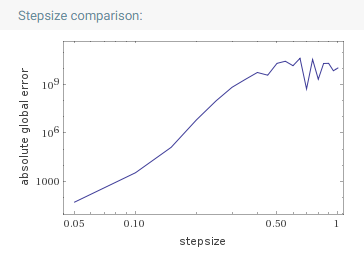
\includegraphics[scale = 0.7]{ComparacionErrorConPaso/errorEuler.png}
        \caption{Gráfico mostrando el error global en función del paso para el método de Euler}
        \label{fig:errorEuler}
    \end{figure}
      
      \newpage

    El paso necesario para que la aproximación numérica obtenida por método de Euler sea comparable a la aproximación del método de Runge-Kutta 4 con $h = 0.02$ es del orden de: $0.0000002$. Como se puede ver en la siguiente figura \footnote{ Lamentablemente no fue posible mostrar la figura donde ambos métodos están superpuestos por problemas técnicos (La computadora no podía calcularlo debido a la cantidad de RAM que necesitaba)}
    

    \begin{figure}[!htb]
        \centering
        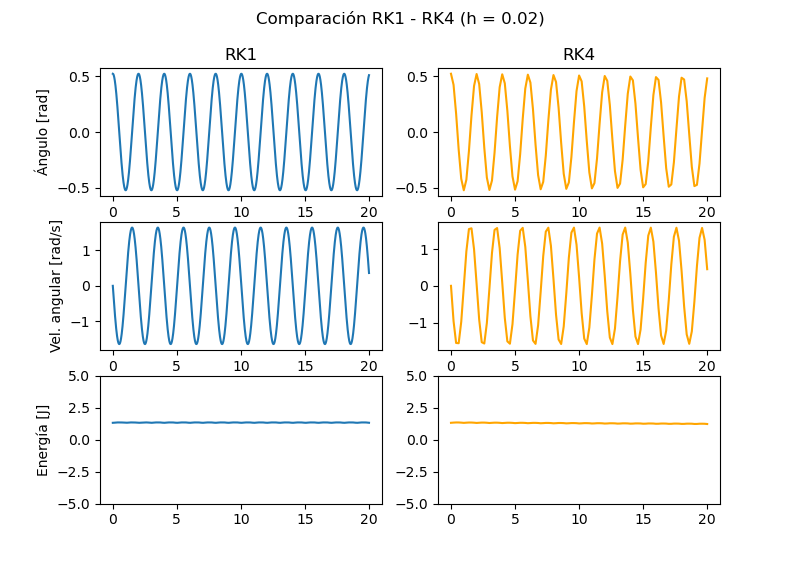
\includegraphics[scale = 0.7]{ambosJuntosSeisCeros.png}
        \caption{Gráfico comparando ambos métodos con distintos pasos}
    \end{figure}

    Esto tiene sentido, pues sabiendo que siendo h = 0.02 y que el error de Runge-Kutta 4 es del orden de $h^{4} = 0.02^{4} \approx 0.0000002$. Entonces dado que el error de Euler es de $O(h)$ entonces es lógico estimar que $h$ para Euler será aproximadamente el conseguido.


\newpage

\subsection{Conclusiones sobre RK4}\label{sec:RK4}
    El método de Runge-Kutta 4 se aproximó a la solución real mucho mejor que el método de Runge-Kutta 1 para todos los pasos h utilizados. Esto era esperable pues el orden de la cota de error total acumulado del método es $0(h^4)$. Esto indica que este método es mejor en el caso general al realizar el cómputo de datos, pues además de ser sencillo es muy preciso.
    
    \begin{figure}[!htb]
        \centering
        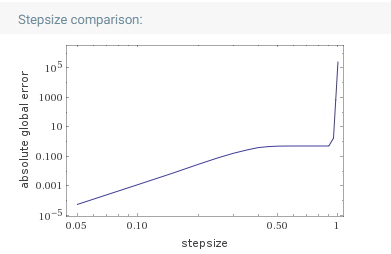
\includegraphics[scale = 0.7]{ComparacionErrorConPaso/errorRK.png}
        \caption{Gráfico mostrando el error global en función del paso para el método de Runge-Kutta 4.}
        \label{fig:errorRK4}
    \end{figure}
    
    Como se pudo observar, para valores de h pequeños y no tan pequeños el método mantiene un error global que consideramos bueno. Pues aún para pasos altos como $h=0.8$ el error es relativamente pequeño.
    
\newpage

\section{Anexo}\label{sec:anexo}
    A continuación, presentamos los gráficos con los que fuimos probando para poder observar dónde ambos métodos coincidían para el caso 1.
    
    Para el caso de h = $0,02$, se puede ver en la figura \ref{fig:noAmortiguadoGrafJuntos}
    
    \begin{figure}[!htb]
        \centering
        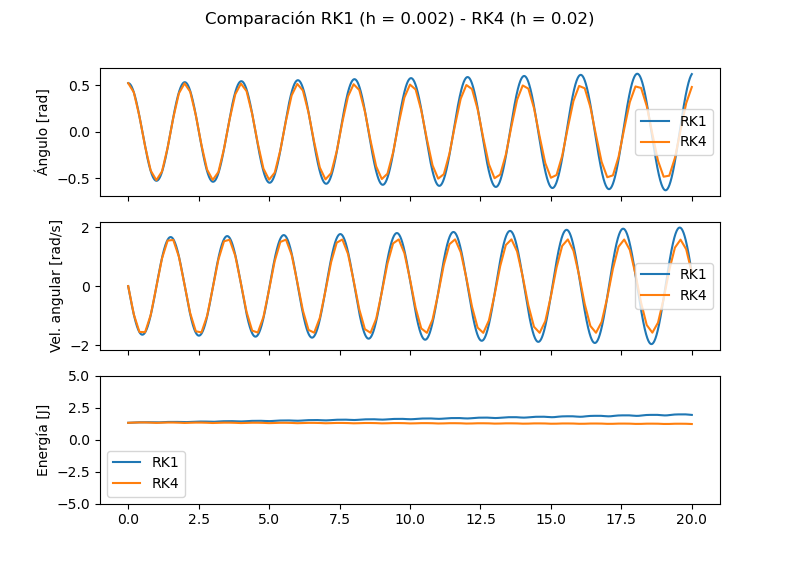
\includegraphics[scale = 0.6]{ambosjuntos 0,002.png}
        \caption{Para $h = 0.002$}
        \label{fig:errorH2}
    \end{figure}
    
    \begin{figure}[!htb]
        \centering
        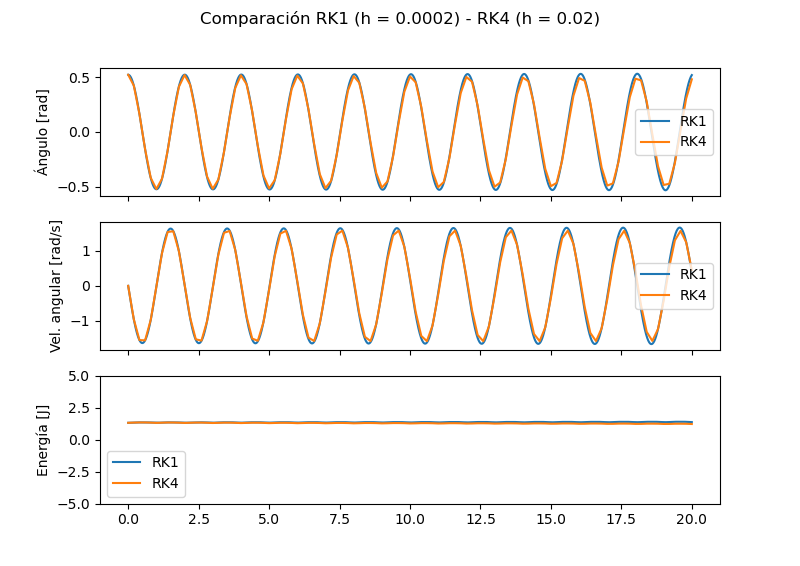
\includegraphics[scale = 0.6]{ambosjuntos 0,0002.png}
        \caption{Para $h = 0.0002$}

    \end{figure}
    
    \begin{figure}[!htb]
        \centering
        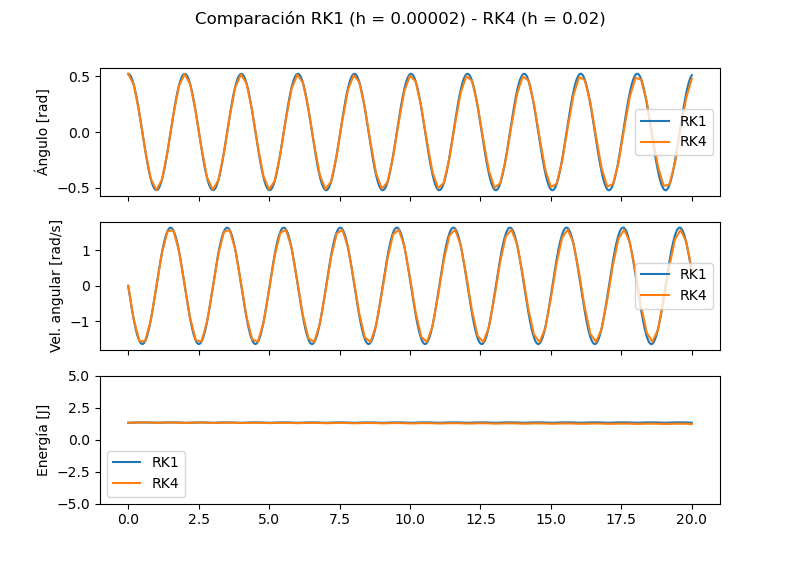
\includegraphics[scale = 0.6]{ambosjuntos 0,00002.png}
        \caption{Para $h = 0.00002$}
        \label{fig:errorH4}
    \end{figure}

    Ya para este último gráfico se puede remarcar el nivel de similitud entre ambos métodos, de aquí se saca la conclusión de que el método de Runge-Kutta 4 es mucho mejor que el método de Euler, pues con muchos menos pasos consigue un mejor resultado.

\section{Bibliografía}\label{sec:bibliografia}

    Ecuaciones Rígidas [1]
    
    \bigskip
    \url{http://www.frsn.utn.edu.ar/gie/an/mnedo/36\_rigidas.html#:~:text=Las\%20ecuaciones\%20r\%C3\%ADgidas\%20son\%20aquellas,que\%20la\%20ecuaci\%C3\%B3n\%20es\%20r\%C3\%ADgida}
    \bigskip
    \url{https://www.researchgate.net/publication/267957513_Comparison_of_Numerical_Methods_for_Solving_Initial_Value_Problems_for_Stiff_Differential_Equations}
    \bigskip
    \url{https://uotechnology.edu.iq/dep-production/branch1_files/Numerical\%20Methods\%20for\%20Ordinary\%20Differential\%20Equations\%20-\%20J.\%20C.\%20Butcher.pdf}

    \bigskip

    Las figuras \ref{fig:errorEuler} y \ref{fig:errorRK4} fueron obtenidas usando WolframAlpha.
    

    %(Para cada caso, compare las curvas de posicion y velocidad angular utilizando ambos metodos, y variando el paso de integracion. Obtenga conclusiones empiricas respecto a como afecta dicho paso a la estimacion de las variables a integrar. Utilice los resultados teoricos de las cotas de error de cada metodo para determinar si sus conclusiones empricas se corres- ponden con las teoricas) PA ESTO HAY QUE COMPARAR CON RK4 CON UN PASO MUUUY CHIQUITO, LA VERDAD DE LA MILANESA . :D
    
\end{document}
